% !TeX root = ../analisi_2.tex

\section{Calcolo differenziale}

\subsection{Derivate parziali e derivate direzionali}

\begin{definition}
Sia $f : A \subseteq \mathbb{R}^2 \to \mathbb{R}$, $A \neq \emptyset$, $A$ aperto.

Sia $(x_0, y_0) \in A$. Allora si chiama \underline{derivata parziale} di $f$ rispetto a $x$ nel pto $(x_0, y_0)$ il seguente limite se $\exists$ finito
\[
\lim_{h \to 0} \frac{f(x_0 + h, y_0) - f(x_0, y_0)}{h}
\]
e si denota con uno dei seguenti:
\[
D_x f(x_0, y_0), \quad f_x(x_0, y_0), \quad \frac{\partial f}{\partial x}(x_0, y_0)
\]
Si chiama \underline{der. parz.} di $f$ rispetto a $y$ nel pto $(x_0, y_0)$ il seguente se $\exists$ finito
\[
\lim_{h \to 0} \frac{f(x_0, y_0 + h) - f(x_0, y_0)}{h}
\]
e si denota con:
\[
D_y f(x_0, y_0), \quad f_y(x_0, y_0), \quad \frac{\partial f}{\partial y}(x_0, y_0)
\]
\end{definition}

$f$ si dice \underline{derivabile in $(x_0, y_0)$} se $\exists$ il vettore
\[
\nabla f(x_0, y_0) = (f_x(x_0, y_0), f_y(x_0, y_0))
\]
\pencilnote{($\nabla$ nabla)} che si chiama \underline{gradiente di $f$ in $(x_0, y_0)$}.

$f$ si dice \underline{derivabile in $A$} se $\exists$ il gradiente in ogni pto.

\begin{example}
\begin{enumerate}
    \item $f(x, y) = x^3 y + \log\left(\frac{x}{y}\right) - 3x^2$

    \begin{center}
    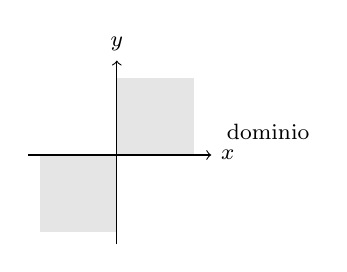
\begin{tikzpicture}[scale=0.75]
        \fill[gray!20] (0,0) rectangle (1.3,1.3);
        \fill[gray!20] (0,0) rectangle (-1.3,-1.3);
        \draw[->] (-1.5,0) -- (1.6,0) node[right] {\footnotesize $x$};
        \draw[->] (0,-1.5) -- (0,1.6) node[above] {\footnotesize $y$};
        \node[right] at (1.7,0.4) {\footnotesize \pencilnote{dominio}};
    \end{tikzpicture}
    \end{center}
    \[
    f_x(x, y) = 3x^2 y + \frac{y}{x} \cdot \frac{1}{y} - 6x
    \]
    \[
    f_y(x, y) = x^3 + \frac{y}{x} \cdot \left(-\frac{x}{y^2}\right) = x^3 - \frac{1}{y}
    \]

    \item $f(x, y) = \sqrt{x^2 + y^2} = \vert (x, y) \vert$
    \[
    f_x(x, y) = \frac{x}{\sqrt{x^2 + y^2}}, \qquad f_y(x, y) = \frac{y}{\sqrt{x^2 + y^2}} \implies \nabla f(x, y) = \frac{(x, y)}{\vert (x, y) \vert}
    \]
    \[
    f_x(0, 0) = \lim_{h \to 0} \frac{f(h, 0) - f(0, 0)}{h} = \lim_{h \to 0} \frac{\vert h \vert}{h} = \nexists
    \]
    \[
    f_y(0, 0) = \lim_{h \to 0} \frac{f(0, h) - f(0, 0)}{h} = \lim_{h \to 0} \frac{\vert h \vert}{h} = \nexists
    \]

    \item $f(x, y) = x\sqrt{y} \qquad y \ge 0$
    \[
    f_x(x, y) = \sqrt{y}, \qquad f_y(x, y) = \frac{x}{2\sqrt{y}} \implies y > 0 \quad \text{\pencilnote{dunque $f_y(x, y)$ è def. in $\mathbb{R}^2 \setminus \{ (x, 0) \}$}}
    \]
    \[
    \frac{\partial f}{\partial y}(0, 0) = \lim_{h \to 0} \frac{f(0, h) - f(0, 0)}{h} = 0
    \]
\end{enumerate}
\end{example}

\begin{oss}
$f$ der. in $(x_0, y_0) \not\implies f$ cont. in $(x_0, y_0)$

\pencilnote{Es.:
\[
f(x, y) = \begin{cases}
\frac{xy}{x^2 + y^2} & \text{se } (x, y) \neq (0, 0) \\
0 & \text{se } (x, y) = (0, 0)
\end{cases}
\]
non è cont. in $(0, 0)$, ma $f_x(0, 0) = \lim_{h \to 0} \frac{f(h, 0) - f(0, 0)}{h} = 0 = f_y(0, 0)$.}
\end{oss}

\begin{definition}
Sia $v = (v_1, v_2)$ una \underline{direzione} ovvero $\vert v \vert = 1$.

Sia $f : A \subseteq \mathbb{R}^2 \to \mathbb{R}$, $A \neq \emptyset$ e aperto e sia $(x_0, y_0) \in A$. Si chiama \underline{derivata direzionale} di $f$ nel pto $(x_0, y_0)$ nella direzione $v$ il seguente limite se $\exists$ finito
\[
\frac{\partial f}{\partial v}(x_0, y_0) = \lim_{h \to 0} \frac{f(x_0 + h v_1, y_0 + h v_2) - f(x_0, y_0)}{h}
\]
\end{definition}

\begin{example}
\[
f(x, y) = \begin{cases}
x e^{\frac{x}{y}} & \text{se } y \neq 0 \\
0 & \text{se } y = 0
\end{cases}
\]
\begin{itemize}
    \item Verificare che $f$ non è continua in $(0, 0)$
    \item $\exists \frac{\partial f}{\partial v}(0, 0) \quad \forall v$
\end{itemize}
\end{example}

\begin{oss}
\underline{L'esistenza di tutte le der. direzionali (lineari), non basta ad implicare la continuità} \pencilnote{(le der. lungo le parabole potrebbero non esistere)}.
\end{oss}

\subsection{Differenziabilità}

\begin{oss}[Idea geometrica]
Sia $f : A \subseteq \mathbb{R}^2 \to \mathbb{R}$, $A \neq \emptyset$, $A$ aperto, e sia $f$ derivabile in un pto $(x_0, y_0) \in A$.

Sezionando il grafico di $f$ con il piano $x = x_0$ si ottiene la curva $z = g(y) = f(x_0, y)$, la cui retta tangente in $y_0$ è
\[
r : \begin{cases}
z = g(y_0) + g'(y_0)(y - y_0) \\
x = x_0
\end{cases}
\implies
\begin{cases}
z = f(x_0, y_0) + \dfrac{\partial f}{\partial y}(x_0, y_0)(y - y_0) \\
x = x_0
\end{cases}
\]
Sezionando con il piano $y = y_0$ si ottiene la curva $z = h(x) = f(x, y_0)$, la cui retta tangente in $x_0$ è
\[
t : \begin{cases}
z = h(x_0) + h'(x_0)(x - x_0) \\
y = y_0
\end{cases}
\implies
\begin{cases}
z = f(x_0, y_0) + \dfrac{\partial f}{\partial x}(x_0, y_0)(x - x_0) \\
y = y_0
\end{cases}
\]
Sia $\pi$ il piano generato da $r$ e $t$, ovvero
\[
\boxed{\pi : z = f(x_0, y_0) + \frac{\partial f}{\partial x}(x_0, y_0)(x - x_0) + \frac{\partial f}{\partial y}(x_0, y_0)(y - y_0)}
\]
\end{oss}

\begin{definition}
Sia $f : A \subseteq \mathbb{R}^2 \to \mathbb{R}$, $A \neq \emptyset$, $A$ aperto, e sia $(x_0, y_0) \in A$.

$f$ si dice \underline{differenziabile} in $(x_0, y_0)$ se:
\begin{enumerate}
    \item $f$ è derivabile in $(x_0, y_0)$, cioè $\exists \nabla f(x_0, y_0)$;
    \item \[
    \lim_{(h, k) \to (0, 0)} \frac{f(x_0 + h, y_0 + k) - f(x_0, y_0) - f_x(x_0, y_0)\, h - f_y(x_0, y_0)\, k}{\sqrt{h^2 + k^2}} = 0
    \]
\end{enumerate}
\end{definition}

La condizione 2) si può riscrivere in modo equivalente:
\begin{align*}
&\iff \lim_{(x, y) \to (x_0, y_0)} \frac{f(x, y) - \left( f(x_0, y_0) + f_x(x_0, y_0)(x - x_0) + f_y(x_0, y_0)(y - y_0) \right)}{\sqrt{(x - x_0)^2 + (y - y_0)^2}} = 0 \quad \text{\pencilnote{(piano $\pi$)}} \\[6pt]
&\iff \lim_{(x, y) \to (x_0, y_0)} \frac{f(x, y) - \left[ f(x_0, y_0) + \langle \nabla f(x_0, y_0), (x - x_0, y - y_0) \rangle \right]}{\sqrt{(x - x_0)^2 + (y - y_0)^2}} = 0 \\[6pt]
&\iff f(x, y) - f(x_0, y_0) - \langle \nabla f(x_0, y_0), (x - x_0, y - y_0) \rangle = o\left( \sqrt{(x - x_0)^2 + (y - y_0)^2} \right)
\end{align*}
\pencilnote{$\implies f(x, y) = f(x_0, y_0) + \langle \nabla f(x_0, y_0), (x - x_0, y - y_0) \rangle + o\left( \sqrt{(x - x_0)^2 + (y - y_0)^2} \right)$, cioè
$\pi : z = f(x_0, y_0) + f_x(x_0, y_0)(x - x_0) + f_y(x_0, y_0)(y - y_0)$.}

\begin{definition}[Piano tangente]
Per definizione data, se $f$ è differenziabile in $(x_0, y_0)$ chiamiamo \underline{piano tangente al grafico di $f$} nel pto $(x_0, y_0, f(x_0, y_0))$ il piano di equazione
\[
z = f(x_0, y_0) + f_x(x_0, y_0)(x - x_0) + f_y(x_0, y_0)(y - y_0)
\]
\end{definition}

\subsubsection*{Il differenziale}

Per la differenziabilità si ha
\[
\underbrace{f(x, y) - f(x_0, y_0)}_{\Delta f} = f_x(x_0, y_0)(x - x_0) + f_y(x_0, y_0)(y - y_0) + o\left( \sqrt{(x - x_0)^2 + (y - y_0)^2} \right)
\]
ovvero, ponendo $x = x_0 + h$, $y = y_0 + k$,
\[
\underbrace{f(x_0 + h, y_0 + k) - f(x_0, y_0)}_{\Delta f(x_0, y_0)} = df(x_0, y_0) + o\left( \sqrt{h^2 + k^2} \right)
\]
dove
\[
df(x_0, y_0) = f_x(x_0, y_0)\, h + f_y(x_0, y_0)\, k
\]
è il \underline{differenziale} di $f$ in $(x_0, y_0)$ \pencilnote{(è una funzione lineare $g(h, k) = ah + bk$ di $(h, k)$)}.

\begin{example}
Sia $f(x, y) = x$. Allora $\nabla f(x_0, y_0) = (1, 0)$ $\forall (x_0, y_0) \in \mathbb{R}^2$ e
\[
df(x_0, y_0) = h \implies dx = h \quad \text{\pencilnote{(non dipende dal punto)}}
\]
Analogamente, se $f(x, y) = y$ allora $dy = k$ \pencilnote{(funzioni proiezione)}.

Allora
\[
\Delta f(x_0, y_0) = f_x(x_0, y_0)\, dx + f_y(x_0, y_0)\, dy + o\left( \sqrt{h^2 + k^2} \right)
\]
cioè
\[
\Delta f(x_0, y_0) = df(x_0, y_0) + o\left( \sqrt{dx^2 + dy^2} \right)
\]
\end{example}

\pencilnote{($df$, $dx$ e $dy$ sono funzionali lineari: $dx$ e $dy$ sono la base canonica dello spazio duale. Vedi bene!)}

\subsection{Differenziabilità e continuità}

\begin{theorem}
Sia $f : A \subseteq \mathbb{R}^2 \to \mathbb{R}$, $A \neq \emptyset$, $A$ aperto.

Se $f$ è differenziabile in $(x_0, y_0)$, allora $f$ è continua in $(x_0, y_0)$.
\end{theorem}

\begin{proof}
Dobbiamo mostrare che $\displaystyle\lim_{(x, y) \to (x_0, y_0)} f(x, y) - f(x_0, y_0) = 0$. Per la differenziabilità:
\[
\lim_{(x, y) \to (x_0, y_0)} f(x, y) - f(x_0, y_0) = \lim_{(x, y) \to (x_0, y_0)} \langle \nabla f(x_0, y_0), (x - x_0, y - y_0) \rangle + o\left( \sqrt{(x - x_0)^2 + (y - y_0)^2} \right)
\]
Ma $\langle \nabla f(x_0, y_0), (x - x_0, y - y_0) \rangle \to 0$ in quanto, per la disuguaglianza di Cauchy--Schwarz,
\[
0 \le \left| \langle \nabla f(x_0, y_0), (x - x_0, y - y_0) \rangle \right| \underset{\text{C.S.}}{\le} \left| \nabla f(x_0, y_0) \right| \cdot \sqrt{(x - x_0)^2 + (y - y_0)^2} \to 0
\]
mentre l'$o(\cdot)$ tende a $0$ per definizione.
\end{proof}

\begin{oss}
\begin{itemize}
    \item $f$ diff. $\implies$ $f$ der. \quad ($\impliedby$ non vale)
    \item $f$ diff. $\implies$ $f$ cont. \quad ($\impliedby$ non vale)
    \item $f$ diff. $\implies$ $\exists \dfrac{\partial f}{\partial v}$ \quad \pencilnote{(?)} \quad ($\impliedby$ non vale)
\end{itemize}
\end{oss}

\subsection{Derivazione delle funzioni composte}

\textbf{Recap:} $f : A \subseteq \mathbb{R}^2 \to \mathbb{R}$, $A \neq \emptyset$, aperto e $f$ diff. e derivabile in $(x_0, y_0)$.
\[
\underbrace{df(x_0, y_0)(h, k)}_{\text{\pencilnote{è un'app. lin.}}} : (h, k) \in \mathbb{R}^2 \to f_x(x_0, y_0)\overbrace{dx}^{h} + f_y(x_0, y_0)\overbrace{dy}^{k} = \Delta f(x_0, y_0) + o\left(\sqrt{(x - x_0)^2 + (y - y_0)^2}\right)
\]

\pencilnote{Si chiamerà ``forma differenziale'' il seguente:
\[
\omega : F_1(x, y)\, dx + F_2(x, y)\, dy
\]}

\begin{theorem}[Der. delle funz. composte]
Sia $f : A \subseteq \mathbb{R}^2 \to \mathbb{R}$, $A \neq \emptyset$ e aperto e sia $\gamma : [a, b] \to A \subseteq \mathbb{R}^2$ e sia $\gamma$ regolare di eq. param. $\gamma(t) = (x(t), y(t))$ e sia $\Gamma$ il suo sostegno ovvero $\gamma([a, b]) = \Gamma \subseteq A$.

Consideriamo $F(t) = f(\gamma(t)) = f(x(t), y(t)) : [a, b] \to \mathbb{R}$.

Allora se $f$ è differenziabile, si ha che $F$ è derivabile e risulta:
\[
\underline{F'(t) = \langle \nabla f(\gamma(t)), \gamma'(t) \rangle} = f_x(x(t), y(t))\, x'(t) + f_y(x(t), y(t))\, y'(t)
\]
\end{theorem}

\begin{proof}
\[
\begin{aligned}
F'(t) &= \lim_{h \to 0} \frac{F(t + h) - F(t)}{h} = \\
&= \lim_{h \to 0} \frac{\overbrace{f(x(t + h), y(t + h)) - f(x(t), y(t))}^{\Delta f}}{h} = \quad \text{\pencilnote{($(x(t), y(t)) = (x_0, y_0)$)}} \\
&= \lim_{h \to 0} \frac{f_x(x(t), y(t))\overbrace{(x(t + h) - x(t))}^{\to x'(t)}}{h} + \\
&\quad + \frac{f_y(x(t), y(t))\overbrace{(y(t + h) - y(t))}^{\to y'(t)}}{h} + \frac{o\left(\sqrt{(x(t + h) - x(t))^2 + (y(t + h) - y(t))^2}\right)}{h} =
\end{aligned}
\]
Devo dim. che $\lim_{h \to 0} \frac{o(\sqrt{u})}{h} = 0 \implies$
\[
\implies \lim_{h \to 0} \underbrace{\frac{o(\sqrt{u})}{\sqrt{u}}}_{\text{\pencilnote{$\to 0$ per def. di $o(u)$}}} \cdot \underbrace{\frac{\sqrt{u}}{h}}_{\text{\pencilnote{devo dim. che sia limitata}}}
\]
Si può scrivere:
\[
\pm \sqrt{\left(\frac{x(t + h) - x(t)}{h}\right)^2 + \left(\frac{y(t + h) - y(t)}{h}\right)^2} \to \pm \sqrt{x'(t)^2 + y'(t)^2} = \pm \vert \gamma'(t) \vert \implies
\]
\[
\implies \lim_{h \to 0} \underbrace{\frac{o(\sqrt{u})}{\sqrt{u}}}_{\text{inf.}} \cdot \underbrace{\frac{\sqrt{u}}{h}}_{\text{limitata}} = 0
\]
\end{proof}

\subsection{Conseguenze e prima interpretazione geometrica del gradiente}

$f$ diff. in $A \subseteq \mathbb{R}^2$, $\vert \nabla f \vert \neq 0$ \pencilnote{(sulla linea di livello)}.

Considero il paraboloide $z = f(x, y) = x^2 + y^2$, $f$ è diff.

\begin{center}
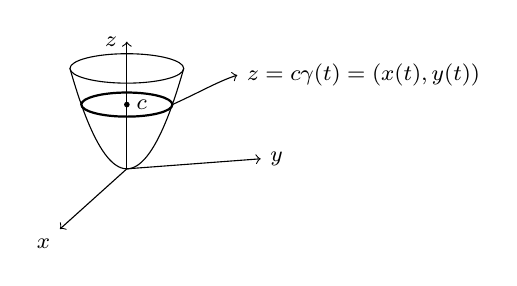
\begin{tikzpicture}[scale=0.85]
    \draw[->] (0,0) -- (-1.0,-0.9) node[below left] {\footnotesize $x$};
    \draw[->] (0,0) -- (2.0,0.15) node[right] {\footnotesize $y$};
    \draw[->] (0,0) -- (0,1.9) node[left] {\footnotesize $z$};
    % Paraboloide con linea di livello z = c
    \draw[domain=-1:1, samples=50] plot ({0.85*\x}, {1.5*\x*\x});
    \draw (0,1.5) ellipse (0.85 and 0.22);
    \draw[thick] (0,0.96) ellipse (0.68 and 0.18);
    \fill (0,0.96) circle (1.2pt) node[right] {\footnotesize $c$};
    \draw[->] (0.68,0.96) .. controls (1.1,1.15) and (1.35,1.3) .. (1.65,1.4) node[right] {\footnotesize $z = c \implies \gamma(t) = (x(t), y(t))$};
\end{tikzpicture}
\end{center}

Sia $\{ f(x, y) = c \}$ una linea di livello:
\[
F(t) = f(\gamma(t)) = c \to F'(t) = 0 \implies \langle \nabla f(\gamma(t)), \gamma'(t) \rangle = 0
\]
Dunque \underline{il gradiente è ortogonale al vett. tang.} \pencilnote{(opp. uno dei due è nullo)}:
\[
\nabla f(\gamma(t)) \perp \gamma'(t)
\]
\pencilnote{(Non mi dà il ``verso'') (Mi dà la direzione).}

\begin{theorem}[Formula del gradiente]
Sia $f : A \subseteq \mathbb{R}^2 \to \mathbb{R}$, $A \neq \emptyset$, aperto, diff. in $(x_0, y_0) \in A$.

Sia $v = (v_1, v_2)$ una direzione di $\mathbb{R}^2$.

Allora $\exists \frac{\partial f}{\partial v}(x_0, y_0)$ e vale:
\[
\boxed{\frac{\partial f}{\partial v}(x_0, y_0) = \langle \nabla f(x_0, y_0), v \rangle = f_x(x_0, y_0)\, v_1 + f_y(x_0, y_0)\, v_2}
\]
\end{theorem}

\begin{proof}
Sia $\gamma(t) = (x_0 + t v_1, y_0 + t v_2)$, $t \in [-\delta, \delta] \implies \gamma'(t) = v$.

$F(t) = f(\gamma(t)) = f(x_0 + t v_1, y_0 + t v_2)$.

Oss. che
\[
\frac{\partial f}{\partial v}(x_0, y_0) \stackrel{?}{=} F'(0) = \lim_{h \to 0} \frac{F(h) - F(0)}{h} = \lim_{h \to 0} \frac{f(x_0 + h v_1, y_0 + h v_2) - f(x_0, y_0)}{h} = \frac{\partial f}{\partial v}(x_0, y_0) \ \checkmark
\]
Quindi $\langle \nabla f(x_0, y_0), \gamma'(0) \rangle = \langle \nabla f(x_0, y_0), v \rangle$.
\end{proof}

\begin{oss}
Dunque:
\begin{itemize}
    \item $f \text{ diff.} \underset{\not\Longleftarrow}{\implies} f \text{ cont.}$
    \item $f \text{ diff.} \underset{\not\Longleftarrow}{\implies} f \text{ der.}$
    \item $f \text{ diff.} \underset{\not\Longleftarrow}{\implies} \exists \frac{\partial f}{\partial v} \quad \forall v$
    \item $f \text{ diff.} \underset{\not\Longleftarrow}{\implies} \text{form. del gradiente}$
    \item $f \text{ diff.} \underset{\not\Longleftarrow}{\implies} \exists \text{ piano tangente}$
\end{itemize}
\end{oss}

\begin{example*}
\pencilnote{
\[
f(x, y) = \begin{cases}
\frac{x^3 y}{x^4 + y^2} & (x, y) \neq (0, 0) \\
0 & \text{altrove}
\end{cases}
\]
Dim. che vale f. del grad. ma non è diff.}
\end{example*}

\subsection{Seconda interpretazione geometrica del gradiente}

$f$ sia diff. in $(x_0, y_0)$, $\vert \nabla f \vert \neq 0$:
\[
\pm v_g = \pm \frac{\nabla f(x_0, y_0)}{\vert \nabla f(x_0, y_0) \vert}
\]
$v_g =$ quella con $+$.
\[
\frac{\partial f}{\partial v_g}(x_0, y_0) = \langle \nabla f(x_0, y_0), v_g \rangle = \vert \nabla f(x_0, y_0) \vert
\]
\[
\frac{\partial f}{\partial (-v_g)}(x_0, y_0) = -\vert \nabla f(x_0, y_0) \vert
\]
Sia $v$ una dir. generica:
\[
\left\vert \frac{\partial f}{\partial v}(x_0, y_0) \right\vert = \vert \langle \nabla f(x_0, y_0), v \rangle \vert \underset{\text{C.S.}}{\le} \vert \nabla f(x_0, y_0) \vert \cdot \underbrace{\vert v \vert}_{= 1}
\]
Dunque
\[
-\vert \nabla f(x_0, y_0) \vert \le \frac{\partial f}{\partial v}(x_0, y_0) \le \vert \nabla f(x_0, y_0) \vert
\]
\[
\frac{\partial f}{\partial (-v_g)}(x_0, y_0) \le \frac{\partial f}{\partial v}(x_0, y_0) \le \frac{\partial f}{\partial v_g}(x_0, y_0) \implies
\]
$\implies$ \underline{La dir. del gradiente è la dir. di massima pendenza}.

\begin{example*}
\pencilnote{
\[
f(x, y) = \begin{cases}
\frac{x^2 y}{x^2 + y^2} & \text{se } (x, y) \neq (0, 0) \\
0 & \text{se } (x, y) = (0, 0)
\end{cases}
\]
Verifica che se è diff. etc.
\begin{enumerate}
    \item $0 \le \frac{\vert x^2 y \vert}{x^2 + y^2} \le \frac{x^2 \vert y \vert}{x^2} \to 0 \implies f$ è cont. in $(0, 0)$.
    \item $\frac{\partial f}{\partial v}(0, 0) = \lim_{h \to 0} \frac{f(h v_1, h v_2) - f(0, 0)}{h} = \lim_{h \to 0} \frac{h^3 v_1^2 v_2}{h^2 \cdot h} = v_1^2 v_2 \implies f_x(0, 0) = 0 = f_y(0, 0)$ (se $v = (1, 0)$ o $(0, 1)$).
\end{enumerate}
Controlla che la f.d.g. non vale $\implies$ non è diff.}
\end{example*}

\subsection{Teorema del differenziale totale}

\begin{theorem}[Teo del differenziale totale]
Sia $f : A \subseteq \mathbb{R}^2 \to \mathbb{R}$, $A \neq \emptyset$ e aperto.

Sia $f$ derivabile in $A$. Sia $(x_0, y_0) \in A$:
\[
\underline{f_x, f_y \text{ siano cont. in } (x_0, y_0) \implies f \text{ è diff. in } (x_0, y_0)}
\]
\end{theorem}

\begin{example*}[Controesempio]
\pencilnote{
\[
f(x, y) = \begin{cases}
y^2 \cos\frac{x}{y} & \text{se } y \neq 0 \\
0 & \text{se } y = 0
\end{cases}
\]
non è $C^1$ ma è diff.}
\end{example*}

\subsection{Teorema di differenziabilità diretta}

\begin{theorem}[Teo differenziabilità diretta]
$f \in C^1(A) \implies f$ è diff. in $A$.
\end{theorem}

\begin{proof}
Scegliamo 1 pto $(x_0, y_0)$ arbitrario $\in A$ e mostriamo che $f$ è diff. in $(x_0, y_0)$.

$\implies$ Per Hp: $f$ è derivabile in $(x_0, y_0)$, quindi devo solo dim.:
\begin{equation*}
\lim_{(h, k) \to (0, 0)} \frac{f(x_0 + h, y_0 + k) - f(x_0, y_0) - f_x(x_0, y_0)\, h - f_y(x_0, y_0)\, k}{\sqrt{h^2 + k^2}} = 0 \tag{I}
\end{equation*}
Questo è vero se e solo se
\begin{equation*}
\lim_{(h, k) \to (0, 0)} \frac{\left| f(x_0 + h, y_0 + k) - f(x_0, y_0) - f_x(x_0, y_0)\, h - f_y(x_0, y_0)\, k \right|}{\sqrt{h^2 + k^2}} = 0 \tag{II}
\end{equation*}
Dimostro che il val. ass. $\to 0$. \pencilnote{($0 \le \text{II} \le ? \implies \text{se } ? \to 0 \text{ ho finito}$)}

Studio
\begin{align*}
f(x_0 + h, y_0 + k) - f(x_0, y_0) &= f(x_0 + h, y_0 + k) + f(x_0, y_0 + k) - f(x_0, y_0 + k) - f(x_0, y_0) = \\
&= \underbrace{f(x_0 + h, y_0 + k) - f(x_0, y_0 + k)}_{\substack{y \text{ è bloccata, mi muovo solo lungo } x \\ g(x) = f(x, y_0 + k)}} + \underbrace{f(x_0, y_0 + k) - f(x_0, y_0)}_{\substack{x \text{ è bloccata} \implies p(y) = f(x_0, y)}} = \\
&= g(x_0 + h) - g(x_0) + p(y_0 + k) - p(y_0) = *
\end{align*}
\pencilnote{Applico Lagrange ad entrambe (per Hp le der. sono cont.):}
\begin{align*}
&\implies \exists x_1 \in [x_0, x_0 + h] : h\, g'(x_1) = g(x_0 + h) - g(x_0) \\
&\implies \exists y_1 \in [y_0, y_0 + k] : k\, p'(y_1) = p(y_0 + k) - p(y_0)
\end{align*}
\[
* = h\, g'(x_1) + k\, p'(y_1) = h\, f_x(x_1, y_0 + k) + k\, f_y(x_0, y_1)
\]
Dunque $\text{II}$ diventa:
\begin{align*}
&\lim_{(h, k) \to (0, 0)} \frac{\left| [f_x(x_1, y_0 + k) - f_x(x_0, y_0)]\, h + [f_y(x_0, y_1) - f_y(x_0, y_0)]\, k \right|}{\sqrt{h^2 + k^2}} \le \\
&\le \lim_{(h, k) \to (0, 0)} \left| f_x(x_1, y_0 + k) - f_x(x_0, y_0) \right| \underbrace{\frac{|h|}{\sqrt{h^2 + k^2}}}_{\le 1} + \left| f_y(x_0, y_1) - f_y(x_0, y_0) \right| \underbrace{\frac{|k|}{\sqrt{h^2 + k^2}}}_{\le 1} \le \\
&\le \lim_{(h, k) \to (0, 0)} \underbrace{\left| f_x(x_1, y_0 + k) - f_x(x_0, y_0) \right|}_{\to 0} + \underbrace{\left| f_y(x_0, y_1) - f_y(x_0, y_0) \right|}_{\to 0} = 0
\end{align*}
\pencilnote{(tutte le der. continue $\implies$ porto il limite ``nella'' funzione)}
\end{proof}

\begin{esercizio}[Studio di funzione]
\[
f(x, y) = e^{2x^2 + y} + \frac{x + 1}{y} \qquad \text{\pencilnote{(nel dominio)}}
\]
Studio in $P = (0, 1)$:
\begin{align*}
f_x(x, y) &= 4x e^{2x^2 + y} + \frac{1}{y} \Bigg|_{(0, 1)} = 1 \\
f_y(x, y) &= e^{2x^2 + y} - \frac{x + 1}{y^2} \Bigg|_{(0, 1)} = e - 1
\end{align*}
\[
\implies \nabla f = (1, e - 1), \qquad |\nabla f| = \sqrt{1 + (e - 1)^2} = \sqrt{2 + e^2 - 2e}
\]
\[
v_g = \frac{\nabla f}{|\nabla f|}
\]
\[
v_g(0, 1) = \left( \frac{1}{\sqrt{e^2 - 2e + 2}}, \frac{e - 1}{\sqrt{e^2 - 2e + 2}} \right)
\]
\end{esercizio}

\subsection{Funzioni a gradiente nullo e Teorema di Lagrange}

\begin{theorem}[Funz. a gradiente nullo in un connesso]
Sia $f : A \subseteq \mathbb{R}^2 \to \mathbb{R}$, $A \neq \emptyset$, aperto e \underline{connesso}.

Sia $f$ deriv. in $A$ con $\nabla f = (0, 0)$ $\forall (x, y) \in A$.

Allora $f$ è \underline{costante}.
\end{theorem}

\begin{proof}
Sia $(x_0, y_0) \in A$.

Sia $(x, y) \neq (x_0, y_0)$, $(x, y) \in A$.

\begin{center}
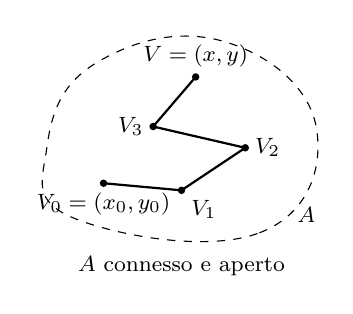
\begin{tikzpicture}[scale=0.9]
    \draw[dashed] plot[smooth cycle, tension=0.75] coordinates {(0,0) (2.6,-0.2) (3.4,1.3) (2.1,2.5) (0.3,2.2) (-0.4,1.0)};
    \node[below right] at (3.0,0.3) {\footnotesize $A$};
    \coordinate (V0) at (0.4,0.5);
    \coordinate (V1) at (1.5,0.4);
    \coordinate (V2) at (2.4,1.0);
    \coordinate (V3) at (1.1,1.3);
    \coordinate (V)  at (1.7,2.0);
    \draw[thick] (V0) -- (V1) -- (V2) -- (V3) -- (V);
    \fill (V0) circle (1.5pt) node[below] {\footnotesize $V_0 = (x_0, y_0)$};
    \fill (V1) circle (1.5pt) node[below right] {\footnotesize $V_1$};
    \fill (V2) circle (1.5pt) node[right] {\footnotesize $V_2$};
    \fill (V3) circle (1.5pt) node[left] {\footnotesize $V_3$};
    \fill (V)  circle (1.5pt) node[above] {\footnotesize $V = (x, y)$};
    \node[below] at (1.5,-0.4) {\footnotesize \pencilnote{$A$ connesso e aperto}};
\end{tikzpicture}
\end{center}

\pencilnote{Per dim. che $f$ è costante, devo dim. che la funz. è costante in quei punti. Dimostriamo che sono connessi per poligonali.}

$V_1 = (x_1, y_1)$ (1° vertice della poligonale), $\gamma(t) = (\text{segmento da } V_0 \text{ a } V_1)$:
\[
\gamma(t) = \begin{cases}
x(t) = x_0 + t(x_1 - x_0) \\
y(t) = y_0 + t(y_1 - y_0)
\end{cases} \qquad t \in [0, 1]
\]
\[
F(t) = f(\gamma(t)) = f(x_0 + t(x_1 - x_0), y_0 + t(y_1 - y_0))
\]
Voglio dim. che la der. è $= 0$ (per dire che è costante):
\[
F'(t) = \langle \underbrace{\nabla f(\gamma(t))}_{= 0}, \gamma'(t) \rangle = 0
\]
Poiché $F'$ è sempre $= 0 \implies F(0) = F(1) \implies f(V_0) = f(V_1)$, cioè $f(x_0, y_0) = f(x_1, y_1)$ \pencilnote{($F$ è costante, quindi lo è anche nei vertici)}.

Ma se con l'Hp che $V_0$ ha un certo val. di $f \implies V_1$ ha lo stesso val. di $f$. Allora con l'Hp che $V_1$ ha una certa $f \implies V_2$ ha la stessa $f \implies \dots \implies$ anche $V$ ha la stessa $f$.
\end{proof}

\begin{example*}[Controesempio]
\[
f(x, y) = \operatorname{arctg} \frac{x}{y} + \operatorname{arctg} \frac{y}{x}
\]
\begin{center}
\begin{tikzpicture}[scale=0.85]
    \draw[dashed, ->] (-1.8,0) -- (1.8,0) node[right] {$x$};
    \draw[dashed, ->] (0,-1.5) -- (0,1.5) node[above] {$y$};
    \node at (0.85,0.75) {\footnotesize $A_1$};
    \node at (-0.85,0.75) {\footnotesize $A_4$};
    \node at (-0.85,-0.75) {\footnotesize $A_3$};
    \node at (0.85,-0.75) {\footnotesize $A_2$};
\end{tikzpicture}
\end{center}
\[
A = A_1 \cup A_2 \cup A_3 \cup A_4 \implies \text{sconnesso}
\]
$\implies$ non si applica il teorema, anche se $\nabla f(x, y) = (0, 0)$.
\end{example*}

\begin{theorem}[Teo di Lagrange]
Sia $f \in C^1(A)$, $A \subseteq \mathbb{R}^2$, $A \neq \emptyset$, aperto.

Siano $P(x_0, y_0)$ e $Q = (x_1, y_1) \in A$ tale che $\overline{PQ} \subseteq A$ \pencilnote{($A$ convesso)}.

Allora $\exists (\bar{x}, \bar{y}) \in A$ (è sul segmento $\overline{PQ}$):
\[
f(Q) - f(P) = \langle \nabla f(\bar{x}, \bar{y}), (x_1 - x_0, y_1 - y_0) \rangle
\]
\pencilnote{DIM (\#todo)}
% #todo: dimostrazione del Teorema di Lagrange nell'ultima pagina
\end{theorem}
